\section{Implementation}

\subsection{Mixed Precision Training}

Mixed precision training uses lower bit floating point types for optimizer states, gradients and model parameters to 
reduce the memory footprint during model training. 

PyTorch offers out-of-the-box support for two types of mixed precision training: Floating point with 16 bits (FP16) and 
brain floating point with 16 bits (BFloat16) which we will introduce in the next sections and explain our integration 
into the OCP project.

\subsubsection{FP16}

FP16 is a floating-point number format which uses 5 bits for the exponent, 10 bits for the fraction and 1 bit for the 
sign. This halves the used memory compared to the default single-precision floating-point format which uses 8 bits 
for the exponent and 24 bits for the fraction. However, FP16 lowers the precision and reduces the range of numbers 
that can be represented, making calculations less accurate and increasing the risk of overflows/underflows.

\begin{figure}[h]
    \centering
    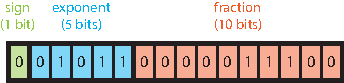
\includegraphics{figures/mixed_precision/float16.pdf}
    \caption{FP16 floating-point number format}
\end{figure}

PyTorch and Deepspeed offer automatic mixed precision for gradients. Developers can regions with context managers 
to allow PyTorch to automatically choose the precision for GPU operations. Unfortunately both autocast modules from 
both PyTorch and Deepspeed failed to detect parameters and gradients in the OCP models when we applied the context 
manager. Our solution was to manually cast parameters to half precision when Deepspeed is used. 

\subsubsection{BFloat16}

As mentioned before, the use of FP16 leads to a higher risk of overflows/underflows. We experienced many overflows 
of gradients when using FP16 with Deepspeed. 

\begin{figure}[h]
    \centering
    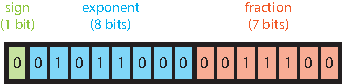
\includegraphics{figures/mixed_precision/bfloat16.pdf}
    \caption{Bfloat16 floating-point number format}
\end{figure}






